% ---------------------------------------------------------------- 3.3 supporting: PM scaling
\begin{frame}{Stage 2, in practice: reward models scale}
\begin{itemize}\itemsep0.3em\small
    \item \emph{Note:} the source paper calls this a ``preference model (PM)'' (the same thing as our \textbf{reward model}).
    \item \textbf{What's measured:} accuracy = how often the model picks the same
          response the human preferred. The axes below are amount of preference data
          (left) and model size (right).
    \item \textbf{Model size} = number of parameters (weights); here $13\text{M}
          \to 52\text{B}$, in $4\times$ steps. \empr{Bigger model + more data $\to$
          a more accurate reward model.}
\end{itemize}
\vfill
\begin{center}
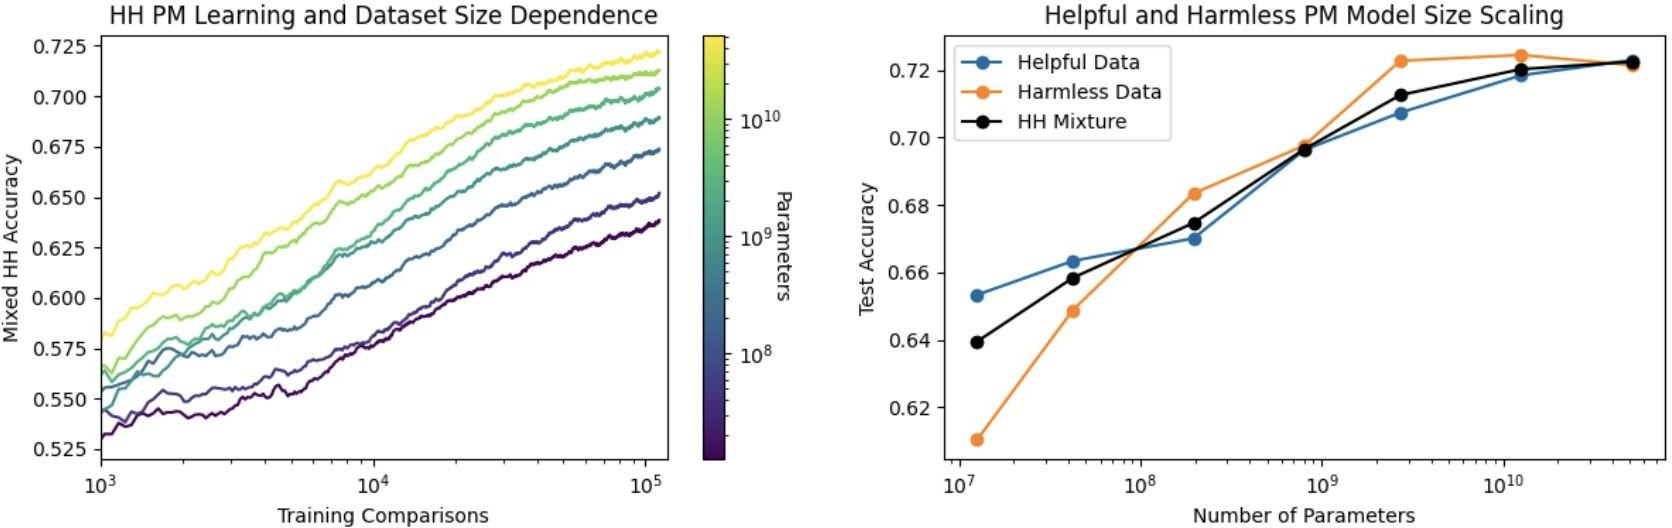
\includegraphics[width=0.78\linewidth, keepaspectratio]{images/rl-real-world/figures/step2-pms.jpg}
\end{center}
\end{frame}

